%\documentclass[12pt, draft]{article}
\documentclass[12pt]{article}
\usepackage{amscd}
\usepackage{amssymb}
\usepackage{mathrsfs}
\usepackage{amsfonts}
\usepackage{mathtools}

\pagestyle{plain}
%\addtolength{\voffset}{1cm}

\usepackage[active]{srcltx}
\usepackage{amsmath,amssymb,amsthm,amsfonts}
%\usepackage{times}
\usepackage{enumerate}
\usepackage{epsfig}
\usepackage{graphicx}
\usepackage{pgf}
\usepackage{subfigure}
%\usepackage{setspace}

\newcommand{\bfmath}[1]{{\mathchoice
    {\mbox{\boldmath$\displaystyle#1$}}
    {\mbox{\boldmath$\textstyle#1$}}
    {\mbox{\boldmath$\scriptstyle#1$}}
    {\mbox{\boldmath$\scriptscriptstyle#1$}}}}
\usepackage[T1]{fontenc}
\usepackage[latin1]{inputenc}
\usepackage[a4paper]{geometry}
%\usepackage{lmodern}
\usepackage[english]{babel}

\newcommand\T{\rule{0pt}{2.6ex}}
\newcommand\B{\rule[-1.2ex]{0pt}{0pt}}

\newcommand{\E}{\mathbb{E}}

\newtheorem{algo}{Algorithm}
\newtheorem*{algo*}{Algorithm}
\newtheorem{remark}{Remark}

\newcommand{\order}{\mathcal{O}}
\textwidth=6.0in
\oddsidemargin=.25in

\def\thesection{\Roman{section}} 

\begin{document}

\begin{figure}
\centering
\subfigure[]{
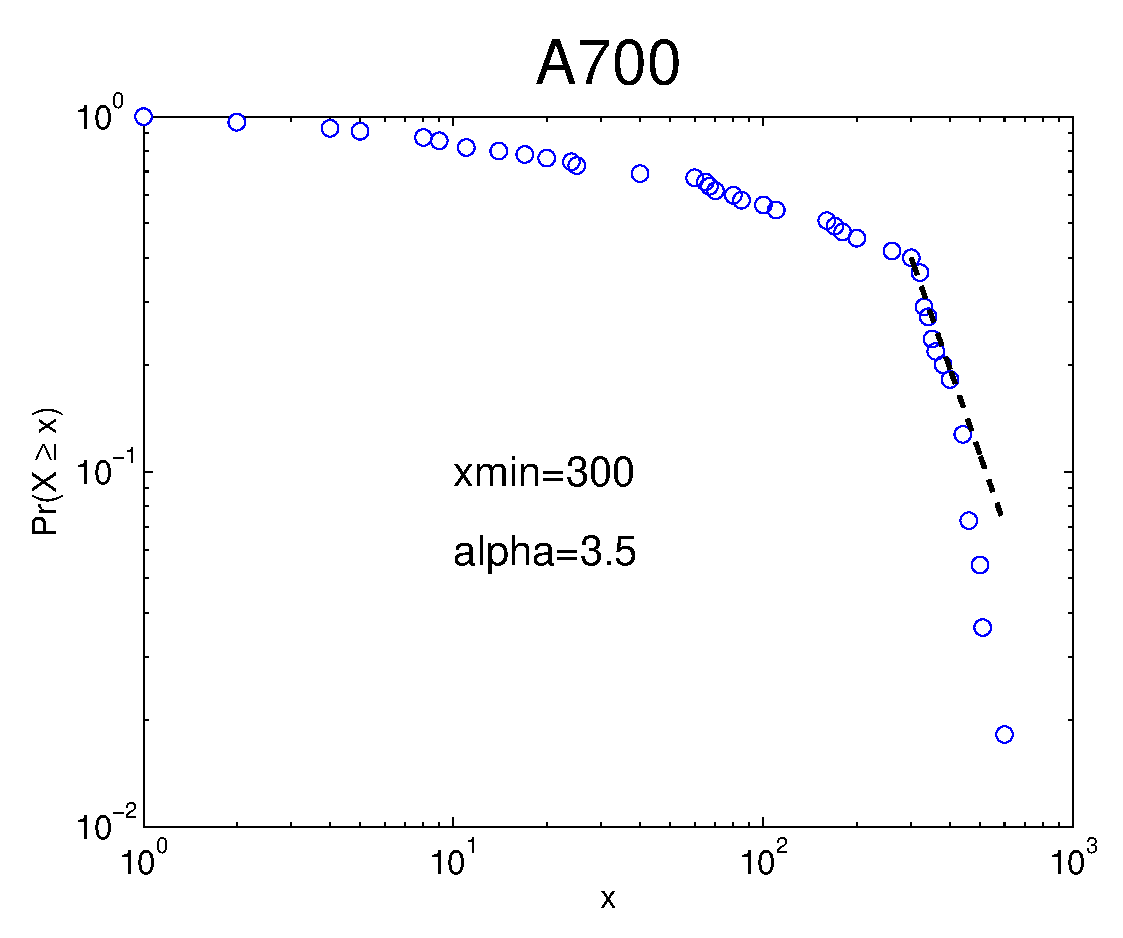
\includegraphics[width=0.3\textwidth]{powertestA700.eps}
}
\subfigure[]{
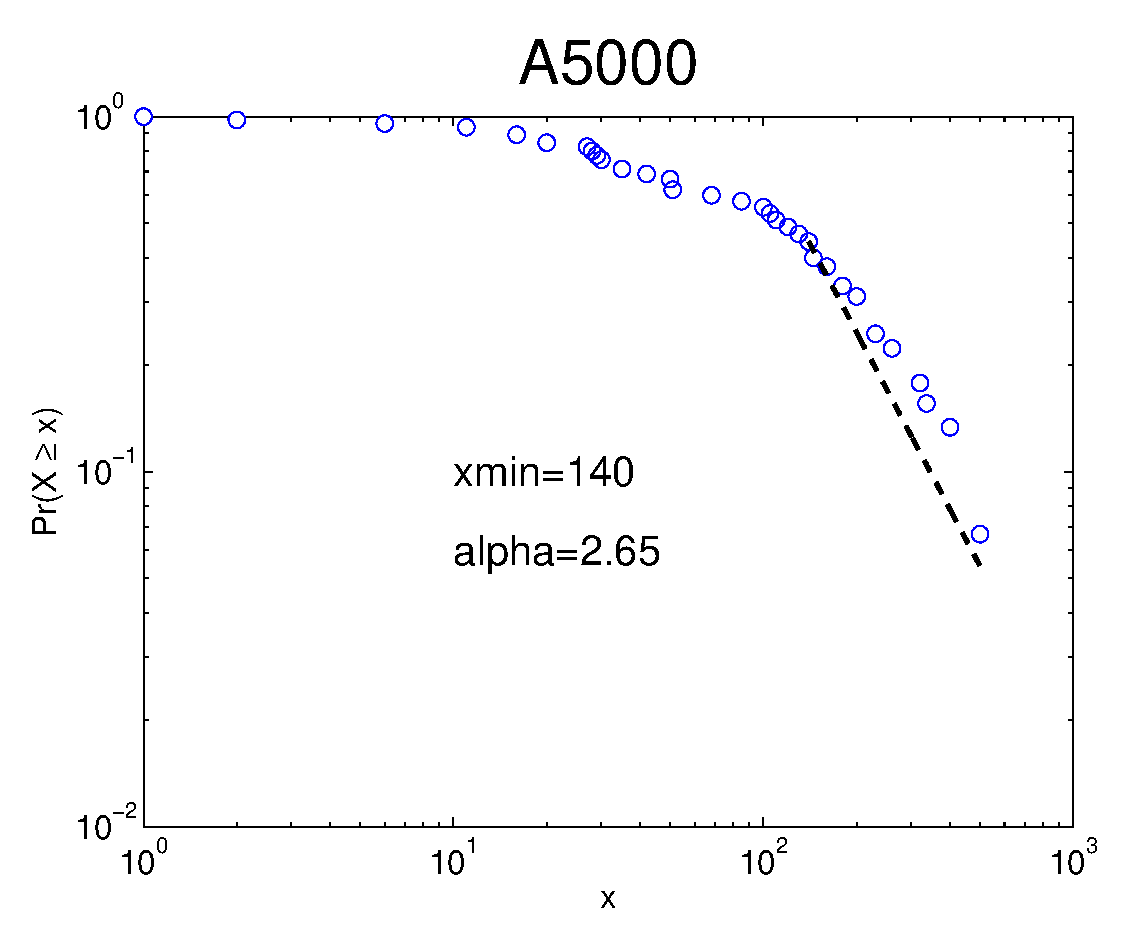
\includegraphics[width=0.3\textwidth]{powertestA5000.eps}
}
\subfigure[]{
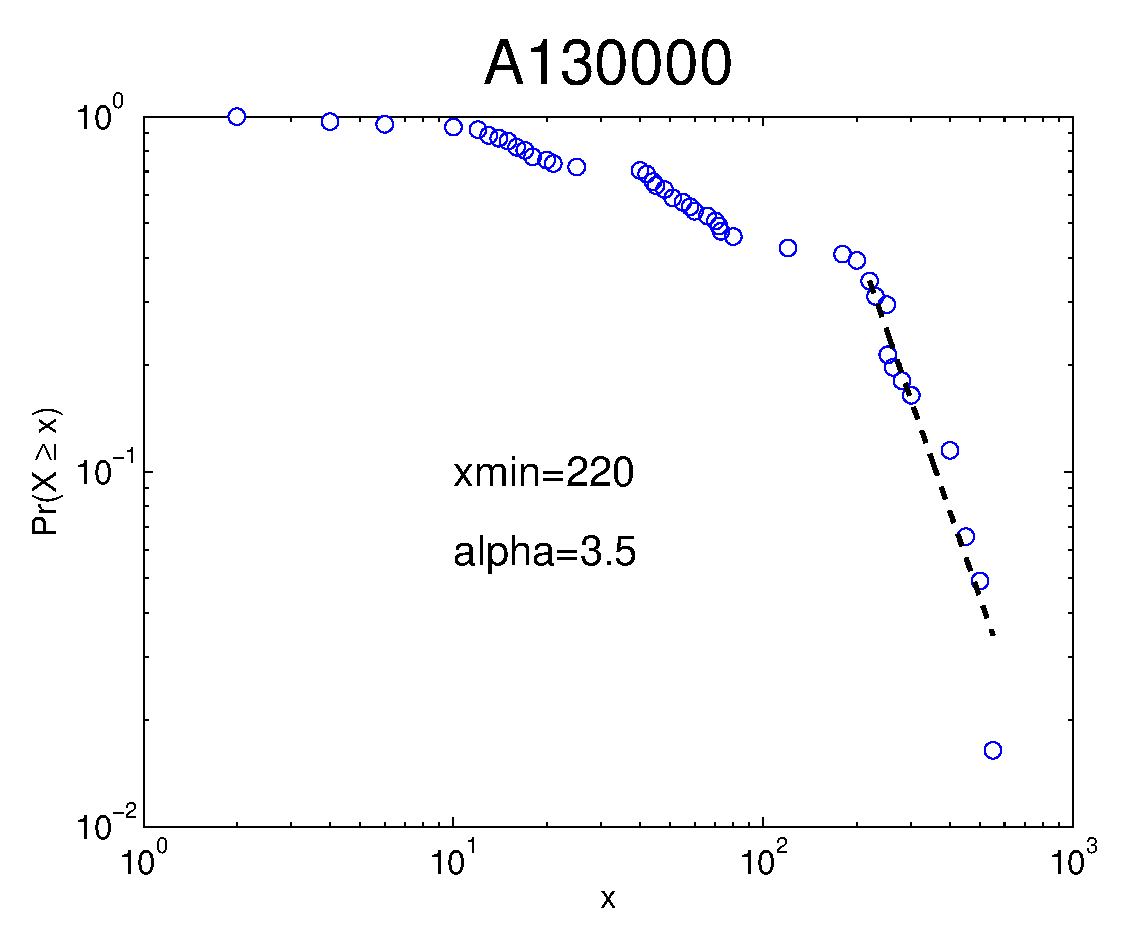
\includegraphics[width=0.3\textwidth]{powertestA130000.eps}
}
\subfigure[]{
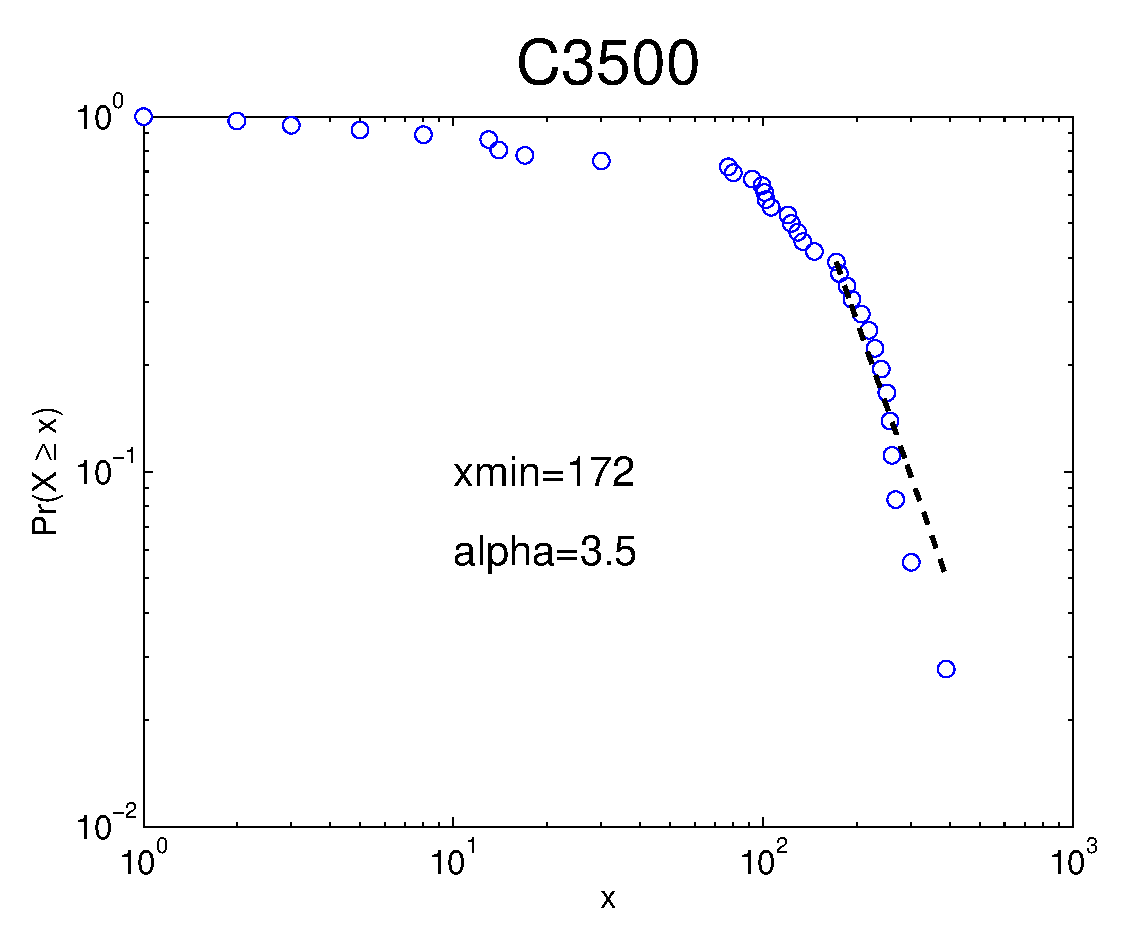
\includegraphics[width=0.3\textwidth]{powertestC3500.eps}
}
\subfigure[]{
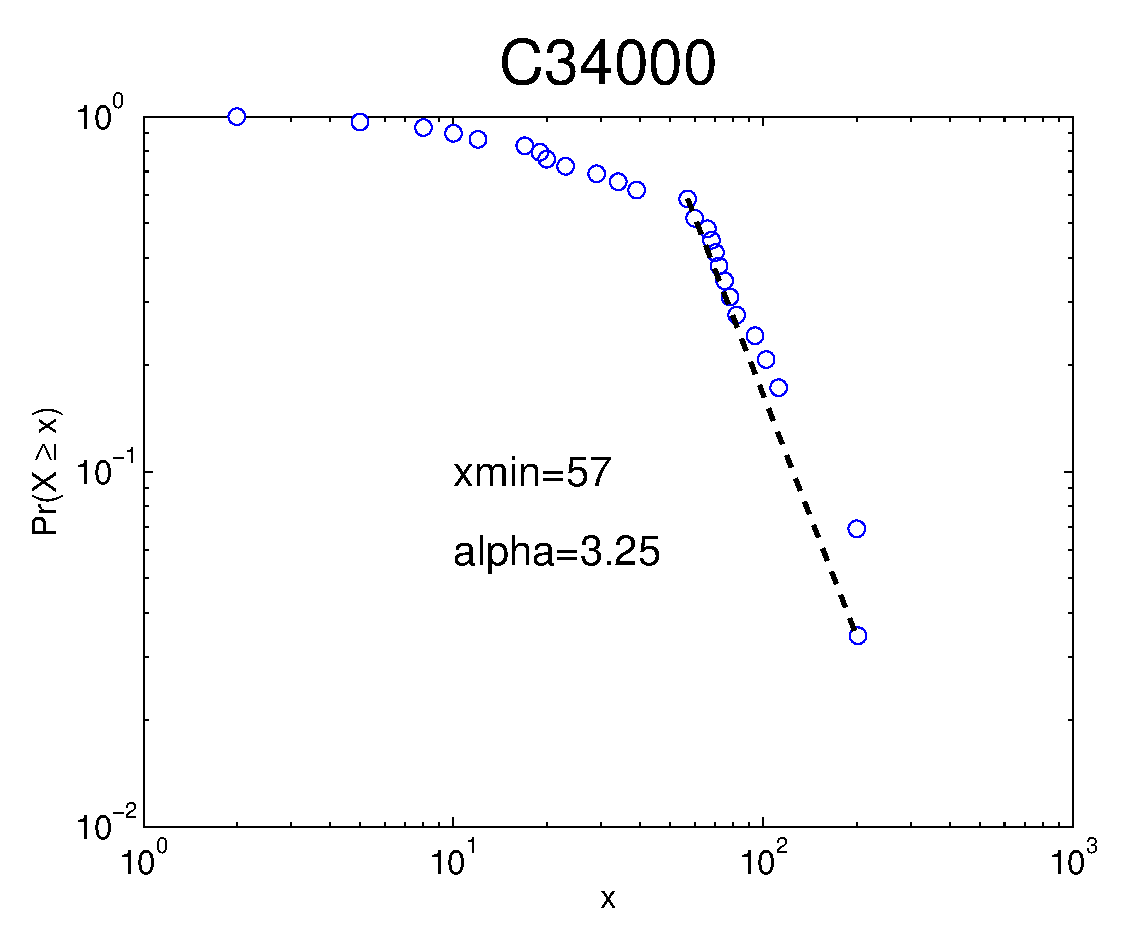
\includegraphics[width=0.3\textwidth]{powertestC34000.eps}
}
\subfigure[]{
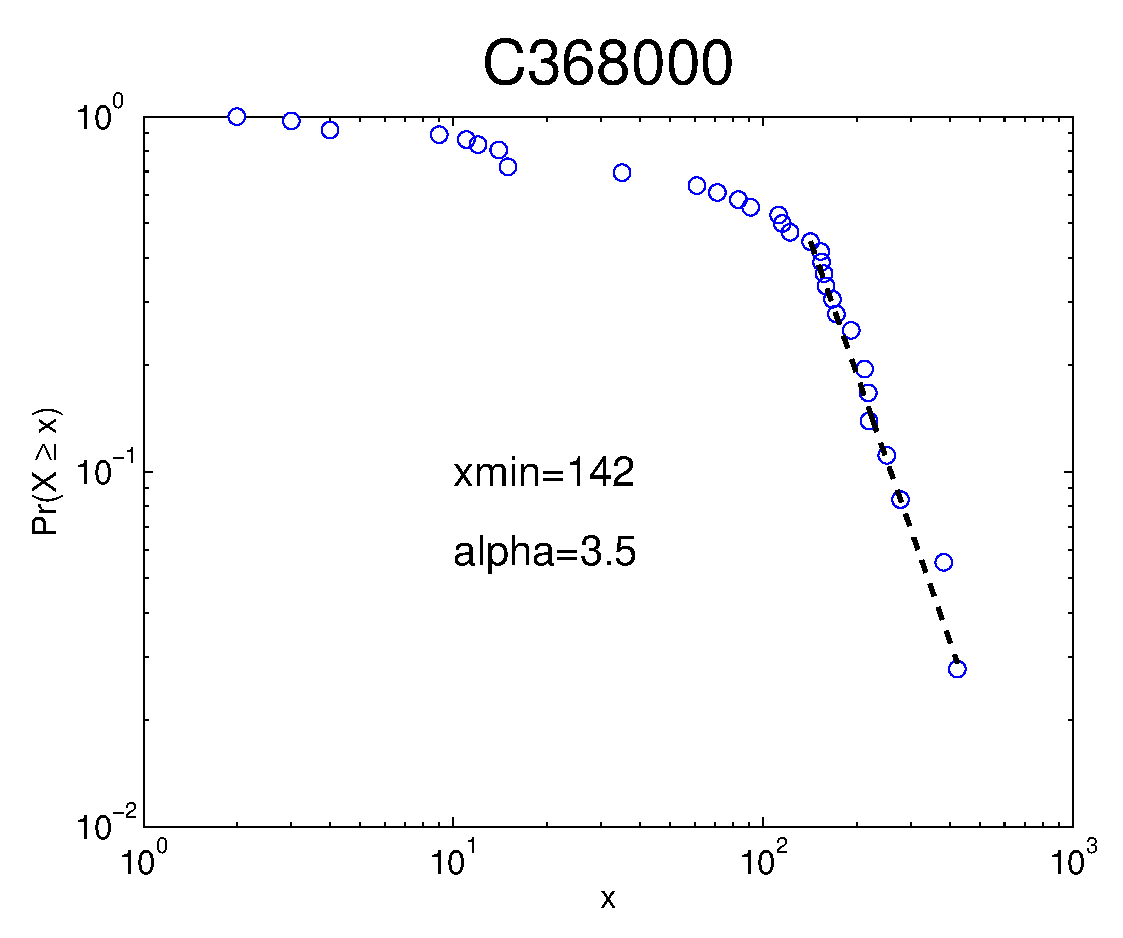
\includegraphics[width=0.3\textwidth]{powertestC368000.eps}
}
\subfigure[]{
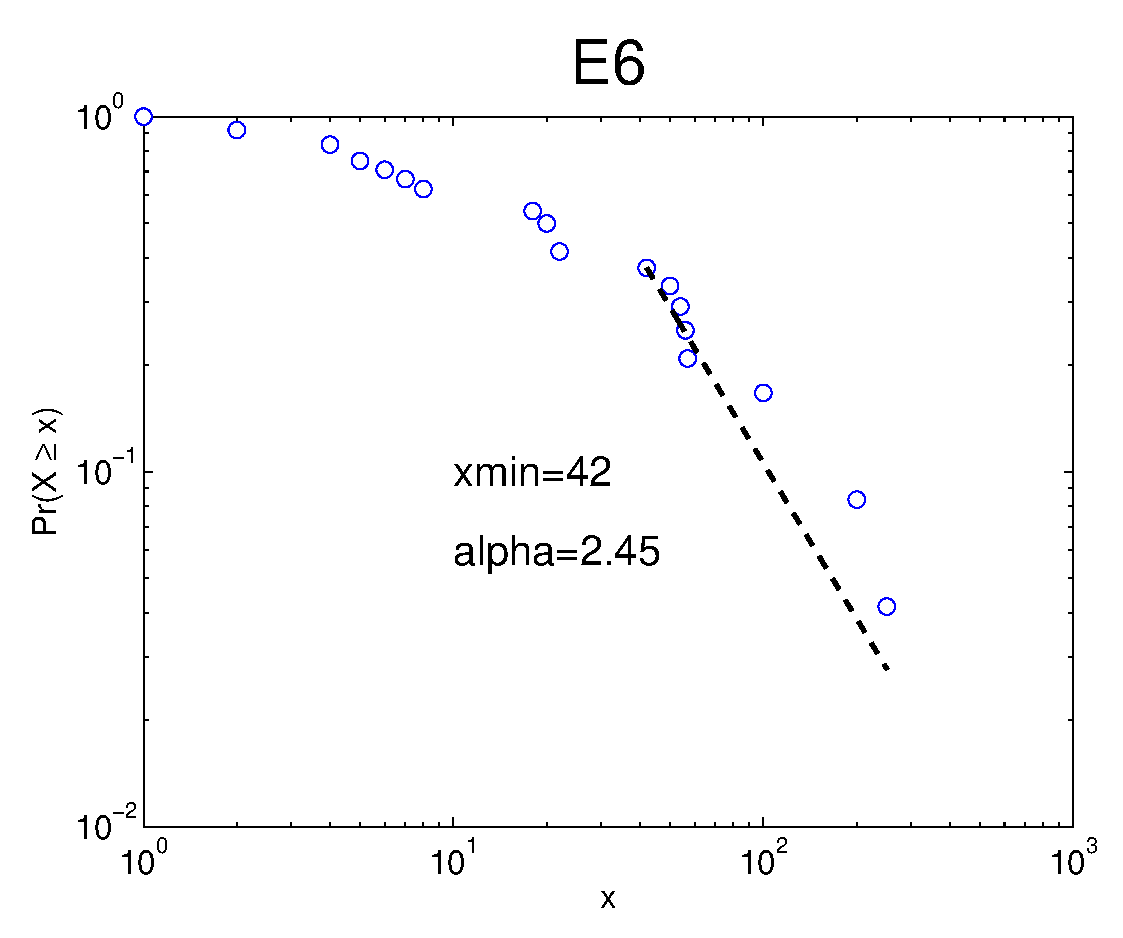
\includegraphics[width=0.3\textwidth]{powertestE6.eps}
}
\subfigure[]{
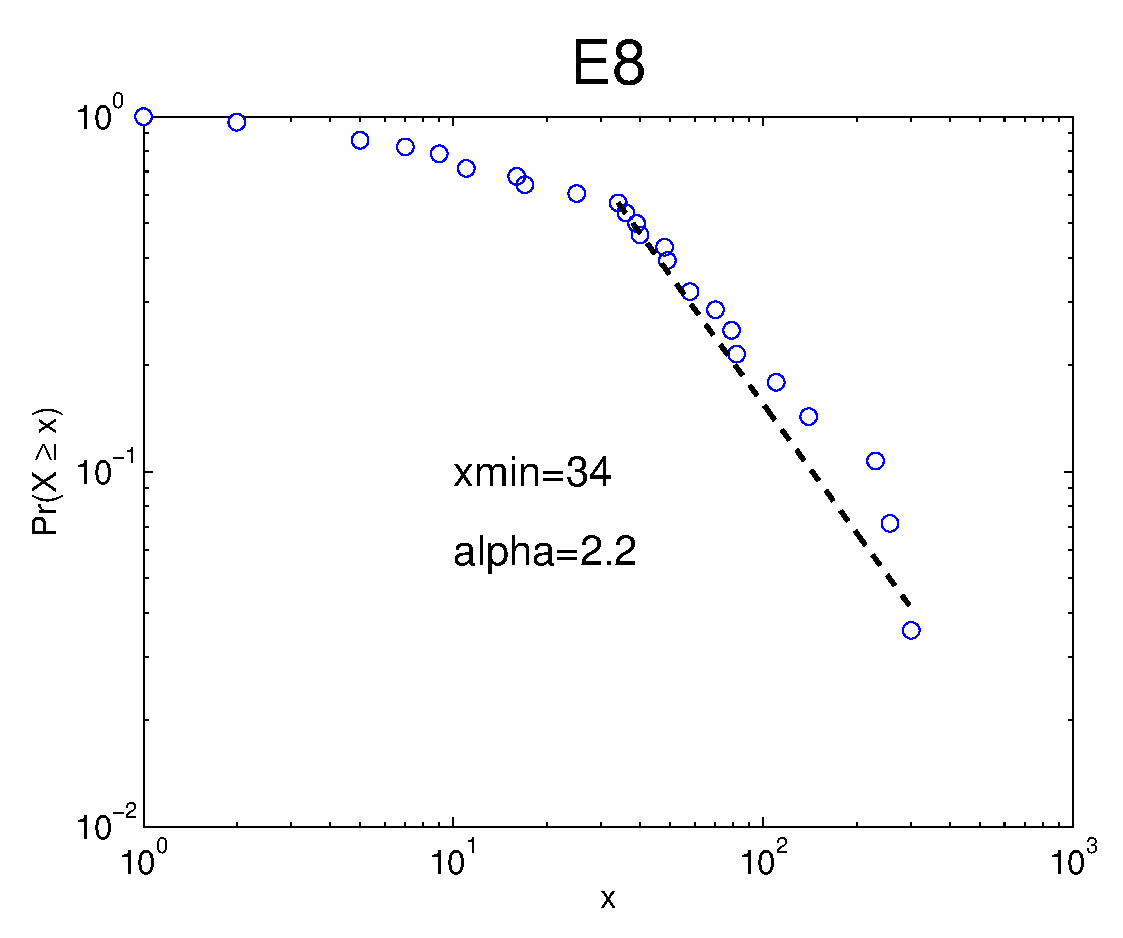
\includegraphics[width=0.3\textwidth]{powertestE8.eps}
}




\end{figure}

\end{document}
